\documentclass[11pt,a4paper]{report}
\usepackage[utf8]{inputenc}
\usepackage[french]{babel}
\usepackage[T1]{fontenc}
\usepackage{amsmath}
\usepackage{amsfonts}
\usepackage{amssymb}
\usepackage{graphicx}
\usepackage[left=2cm,right=2cm,top=2cm,bottom=2cm]{geometry}
\begin{document}
\title{Rapport laboratoire de mesure}
\chapter{Définition}	
\section{But}

Le but de cette manipulation est d'analyser l'influence d'une charge placée sur une balance et sur le pont de Wheatstone via des capteurs de déformations.La Jauge de déformation a donc pour but de traduire la déformation d'une pièce en variation de résistance électrique.Les différentes grandeurs d'influences devra ainsi être analysées comme l'excentration de la charge sur la mesure et de manière théorique, l'influence de la température sur le système.
\section{Hypothèse}

\subsection{Formule1}
\subsection{Formule2}
\section{Schema fonctionnel}
\begin{center}
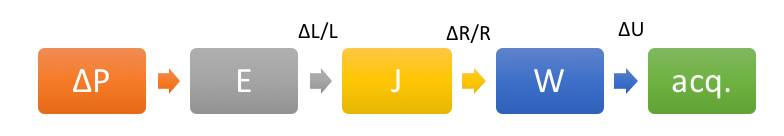
\includegraphics[scale=0.5]{image1.jpg} 
\end{center}

Losqu'on applique un effort F au capteur, un champ de contrainte apparait et donc des déformations apparaissent.Le corps d'épreuve est en effet soumis à allongement suivant l'axe radial du fait par compression(Loi de Hooke) d'une autre part nous avons un allongement suivant l'axe latéral qui va rétrécir le diamètre de la pièce (Coefficient de Poisson) Grâce à la loi de Pouillet , nous pourrons connaitre la variation de la résistance dans le fil.Nous pouvons négligé la résistivité ainsi que le volume. On introduit alors K qui est le facteur de jauge qui caractérise la variation résistance en fonction de sa déformation axiale.Nous avons ici de très petites variations de résistance.
C'est pourquoi, la mesure ne peut s'effectuer directement avec un ohmètre.L'utilisation d'un pont de Wheatstone va permettre de mesurer de telles variations.Soit, un circuit constitué de 4 résistances montées en pont dans lequel on l'a alimenté sous une tension de 5V. A l'équilibre la tension de sortie est nulle mais la variation d'une quelconque des résistances va faire apparaître une différence de potentiel.La tension de sortie est donc proportionnel aux variations relatives deltaR/R de chacune des résistances. 

\chapter{Liste du matériel}
\begin{itemize}
\item poids 
\item corps d'épreuve
\end{itemize}	

\chapter{Procédure}

\chapter{Mesures \& observations}
\section{Graphique}
\section{Tableau de valeurs}

	
\chapter{Interpretation}	
\chapter{Conclusion}	
\chapter{Annexe}	



\end{document}